\chapter{种群遗传学与自然选择}\label{ch:b2:population-genetics}

1848 年，人们在曼彻斯特附近捕到一只黑色的胡椒蛾；到 1895 年，
该市每二十只蛾中就有十九只是黑色的，到 1970 年，随着煤烟
散去，浅色型又回来了。蛾本身并没有改变：
改变的是数以百万计个体的种群中两个\omterm{def:b2:meiosis-heredity:vocabulary}{等位基因}的比例，
而这一切发生在鸟类的注视之下，仅用了几十代。达尔文早已看出
自然选择必然改变物种，却没有办法计量它；这种计量
正是\omterm{def:b2:population-genetics:frequencies}{种群遗传学}，它就是本章的运算。本章要问的是，
在无任何作用时\omterm{def:b2:population-genetics:frequencies}{等位基因频率}如何表现，
然后选择、\omterm{def:b2:genome-diversification:mutation}{突变}、迁移、机遇与\omterm{prop:b2:population-genetics:inbreeding}{近交}各以怎样的速度推动它们变化，
并以性状收尾——这些性状并非一个基因、而是许多基因所决定，
而它们恰恰是自然选择实际所作用的大部分对象，
即自然选择所“看到”的东西。

\section{静止状态下的基因库}

\begin{definition}[种群、基因库、频率]\label{def:b2:population-genetics:frequencies}
\index{种群遗传学}\index{基因库}\index{等位基因频率}
称\emph{种群}为同一物种中能够相互交配的一群个体，
其\emph{基因库}是这些个体全部\omterm{def:b2:meiosis-heredity:vocabulary}{等位基因}的集合。
对于\omterm{def:b2:meiosis-heredity:meiosis}{二倍体}种群中一个具有两个\omterm{def:b2:meiosis-heredity:vocabulary}{等位基因} $A$ 和 $a$ 的基因座，设该种群含
$N$ 个个体，则\emph{\omterm{def:b2:meiosis-heredity:vocabulary}{等位基因}频率}为 $p = (2N_{AA} +
N_{Aa})/2N$，及 $q = 1 - p$，而\emph{\omterm{def:b2:meiosis-heredity:vocabulary}{基因型}频率}是
$AA$、$Aa$ 和 $aa$ 各自所占的比例。从最狭义上说，演化
就是\omterm{def:b2:meiosis-heredity:vocabulary}{等位基因}频率在各代之间的变化；本章的
问题是什么在改变它们，以及改变多少。
\end{definition}

\begin{theorem}[哈代–温伯格]\label{thm:b2:population-genetics:hw}
\index{哈代–温伯格定律}
在随机交配的大种群中，若无选择、\omterm{def:b2:genome-diversification:mutation}{突变}
或迁移，则\omterm{def:b2:population-genetics:frequencies}{等位基因频率}在代与代之间
不发生变化，且经过一代随机交配后，
\omterm{def:b2:meiosis-heredity:vocabulary}{基因型}频率为
\[
AA : p^{2}, \qquad Aa : 2pq, \qquad aa : q^{2},
\]
并保持此比例不变。\omterm{def:b2:meiosis-heredity:vocabulary}{显性}并不会使\omterm{def:b2:meiosis-heredity:vocabulary}{显性}\omterm{def:b2:meiosis-heredity:vocabulary}{等位基因}扩散，并且
罕见的\omterm{def:b2:meiosis-heredity:vocabulary}{隐性}\omterm{def:b2:meiosis-heredity:vocabulary}{等位基因}也不会丢失：它隐藏于\omterm{def:b2:meiosis-heredity:vocabulary}{杂合}子之中，
\omterm{def:b2:meiosis-heredity:vocabulary}{杂合}子与\omterm{def:b2:meiosis-heredity:vocabulary}{纯合}子之比为 $2p/q$ 比 1——当 $q = 0.01$ 时，
即两百比一。该定律是\omterm{def:b2:population-genetics:frequencies}{种群遗传学}的
原假设：真实种群中对它的偏离，或
$p$ 在代际间的变化，即为以下诸作用力之一的
标志。
\end{theorem}
\begin{proof}
随机交配就是配子的随机结合：一个配子携带 $A$ 的
概率为 $p$，携带 $a$ 的概率为 $q$，与其配偶无关。
因此合子为 $AA$ 的概率为 $p^{2}$，$Aa$ 的
概率为 $2pq$，$aa$ 的概率为 $q^{2}$。下一代的\omterm{def:b2:population-genetics:frequencies}{等位基因
频率}为 $p' = p^{2} + \tfrac12(2pq) = p(p + q) = p$，保持不变。
由于\omterm{def:b2:meiosis-heredity:vocabulary}{基因型}频率只依赖于 $p$，它们与
此后每一代都保持相同。
\end{proof}

\begin{example}[读懂一个频率]\label{ex:b2:population-genetics:cf}
囊性纤维化为\omterm{def:b2:meiosis-heredity:vocabulary}{隐性}遗传病，每 2500 名欧洲儿童中有一人患病：
$q^{2} = 1/2500$，$q = 0.02$，携带者频率为 $2pq
\approx 0.04$——即每 25 人中有一人携带一个会使其
\omterm{def:b2:meiosis-heredity:vocabulary}{纯合}子致死的\omterm{def:b2:meiosis-heredity:vocabulary}{等位基因}，而该\omterm{def:b2:meiosis-heredity:vocabulary}{等位基因}有 \qty{98}{\%} 的拷贝位于
健康携带者体内，选择察觉不到它们。这就是
致死性\omterm{def:b2:meiosis-heredity:vocabulary}{隐性}\omterm{def:b2:meiosis-heredity:vocabulary}{等位基因}被清除得如此缓慢的原因，也是
通过绝育患者来消除\omterm{def:b2:meiosis-heredity:vocabulary}{隐性}疾病的优生方案从来都
不可能奏效：下一节的运算将说明这一过程的
缓慢程度。
\end{example}

\section{选择}

\begin{definition}[适合度]\label{def:b2:population-genetics:fitness}
\index{适合度}\index{选择系数}
某\omterm{def:b2:meiosis-heredity:vocabulary}{基因型}的\emph{适合度} $w$ 是其对下一代的相对
后代贡献——即存活至繁殖的概率，
乘以繁殖力，并使最佳\omterm{def:b2:meiosis-heredity:vocabulary}{基因型}的 $w = 1$。
\emph{选择系数} $s$ 是该\omterm{def:b2:meiosis-heredity:vocabulary}{基因型}的亏缺，
$w = 1 - s$。适合度是\omterm{def:b2:meiosis-heredity:vocabulary}{基因型}在某一环境中的性质，
而非\omterm{def:b2:meiosis-heredity:vocabulary}{等位基因}本身的属性：黑化蛾的\omterm{def:b2:meiosis-heredity:vocabulary}{等位基因}在烟尘\omterm{def:b2:plant-meristems:wood}{树皮}上具有 $w > 1$，
相对于浅色型，而在地衣上则具有 $w < 1$。
\end{definition}

\begin{theorem}[选择改变等位基因频率]\label{thm:b2:population-genetics:selection}
\index{自然选择!方程}
设\omterm{def:b2:meiosis-heredity:vocabulary}{基因型}\omterm{def:b2:population-genetics:fitness}{适合度}为 $w_{AA}$、$w_{Aa}$、$w_{aa}$，则平均
\omterm{def:b2:population-genetics:fitness}{适合度}为 $\bar w = p^{2}w_{AA} + 2pq\,w_{Aa} + q^{2}w_{aa}$，而下一代的
\omterm{def:b2:population-genetics:frequencies}{等位基因频率}为
\[
p' = \frac{p^{2}w_{AA} + pq\,w_{Aa}}{\bar w}, \qquad
\Delta p = p' - p = \frac{pq\,\bigl[p(w_{AA} - w_{Aa}) + q(w_{Aa} - w_{aa})\bigr]}{\bar w}.
\]
由此可得两条推论。第一，$\Delta p$ 与 $pq$ 成正比：选择
在中等频率时最快，
而\omterm{def:b2:meiosis-heredity:vocabulary}{等位基因}罕见或近乎固定时最慢——此时可供作用的变异很少。
第二，对于\omterm{def:b2:meiosis-heredity:vocabulary}{隐性}\omterm{def:b2:meiosis-heredity:vocabulary}{等位基因}（$w_{AA} = w_{Aa} = 1$，$w_{aa} =
1 - s$）时，变化量为 $\Delta q = -s\,pq^{2}/\bar w$，与
$q^{2}$ 成正比：罕见的\omterm{def:b2:meiosis-heredity:vocabulary}{隐性}\omterm{def:b2:meiosis-heredity:vocabulary}{等位基因}几乎不被选择察觉，而
将其频率由 $0.01$ 减半约需一百代，
即使其\omterm{def:b2:meiosis-heredity:vocabulary}{纯合}子致死。有利的\omterm{def:b2:meiosis-heredity:vocabulary}{显性}\omterm{def:b2:meiosis-heredity:vocabulary}{等位基因}
起初扩散很快，而在末期停滞，
道理相同。
\end{theorem}
\begin{proof}
在后代中，占比 $p^{2}w_{AA}/\bar w$ 的为 $AA$，
占比为 $2pq\,w_{Aa}/\bar w$ 的为 $Aa$（各\omterm{def:b2:meiosis-heredity:vocabulary}{基因型}的频率按其\omterm{def:b2:population-genetics:fitness}{适合度}加权
并归一化）：其中 $A$ \omterm{def:b2:meiosis-heredity:vocabulary}{等位基因}全部来自第一类，
一半来自第二类，由此得到 $p'$。减去 $p =
p\bar w/\bar w$ 并展开 $\bar w$，即得 $\Delta p$。对于致死的
\omterm{def:b2:meiosis-heredity:vocabulary}{隐性}\omterm{def:b2:meiosis-heredity:vocabulary}{等位基因}（$s = 1$）：$q' = q^{2}\cdot 0 + pq$ 除以 $\bar w = 1 -
q^{2}$，故 $q' = q/(1 + q)$，从而 $1/q' = 1/q + 1$，经过 $t$
代后有 $1/q_t = 1/q_0 + t$：从 $q_0 = 0.01$ 降到 $0.005$ 需要
$t = 100$。
\end{proof}

\begin{omfigure}
\begin{tikzpicture}
\begin{axis}[
  width=0.8\linewidth, height=6cm,
  axis x line=bottom, axis y line=left,
  xmin=0, xmax=150, ymin=0, ymax=1.05,
  xlabel={代数}, ylabel={优势等位基因频率},
  xlabel style={font=\small, at={(axis description cs:0.5,-0.11)}, anchor=north},
  ylabel style={font=\small},
  tick label style={font=\small}, xtick={0,50,100,150}, ytick={0,0.5,1},
  legend style={font=\scriptsize, at={(0.97,0.35)}, anchor=east, draw=none},
  clip=false,
]
\addplot[very thick, omDef] table[x=t, y=dom] {
t dom
0 0.01
10 0.02
20 0.04
30 0.075
40 0.14
50 0.24
60 0.38
70 0.53
80 0.66
90 0.76
100 0.83
110 0.88
120 0.91
130 0.93
140 0.945
150 0.955
};
\addlegendentry{优势等位基因为显性，$s = 0.1$}
\addplot[very thick, omThm] table[x=t, y=rec] {
t rec
0 0.01
10 0.0101
20 0.0102
30 0.0104
40 0.0106
50 0.0108
60 0.011
70 0.0113
80 0.0116
90 0.012
100 0.0124
110 0.0128
120 0.0133
130 0.0138
140 0.0144
150 0.015
};
\addlegendentry{优势等位基因为隐性，$s = 0.1$}
\end{axis}
\end{tikzpicture}

{\small 自然选择的作用，优势为 \qty{10}{\%}。一个有利的
\omterm{def:b2:meiosis-heredity:vocabulary}{显性}\omterm{def:b2:meiosis-heredity:vocabulary}{等位基因}由 \qty{1}{\%} 在七十
代内升至多数，随后增速放缓，其罕见的\omterm{def:b2:meiosis-heredity:vocabulary}{隐性}对手
藏身于\omterm{def:b2:meiosis-heredity:vocabulary}{杂合}子之中；处于 \qty{1}{\%} 的有利\omterm{def:b2:meiosis-heredity:vocabulary}{隐性}\omterm{def:b2:meiosis-heredity:vocabulary}{等位基因}
在同一时间内几乎不动，因为它很少暴露出来。}
\end{omfigure}

\begin{proposition}[选择的类型]\label{prop:b2:population-genetics:kinds}
\index{定向选择}\index{稳定选择}\index{平衡选择}\index{杂合子优势}
\emph{定向}选择偏向一个极端，使一个\omterm{def:b2:meiosis-heredity:vocabulary}{等位基因}趋向
固定（煤烟林中的黑化蛾；抗生素
抗性；干旱时雀喙的大小）。
\emph{稳定}选择偏向中间，淘汰
两端（人类出生体重：死亡的婴儿是最轻的
和最重的）；它使种群保持现状，是
最常见的一类。\emph{分裂}选择偏向两个极端，
不利于中间类型，可使种群分裂
（见\cref{ch:b2:speciation}）。\emph{平衡}选择使两个
\omterm{def:b2:meiosis-heredity:vocabulary}{等位基因}在种群中无限期保留：通过\emph{\omterm{prop:b2:population-genetics:kinds}{杂合子
优势}}，当 $Aa$ 比任一\omterm{def:b2:meiosis-heredity:vocabulary}{纯合}子更适合——其中
$w_{AA} = 1 - s$，$w_{aa} = 1 - t$，$w_{Aa} = 1$，频率趋于
$\hat p = t/(s + t)$——或通过\emph{频率依赖}
选择，即某一\omterm{def:b2:meiosis-heredity:vocabulary}{基因型}越稀有越适合（稀有的
在\cref{ch:b2:angiosperm-reproduction}中的 $S$ \omterm{def:b2:meiosis-heredity:vocabulary}{等位基因}，被捕食者
未学会识别的猎物，以及食鳞鱼的
左右两型口）。
\end{proposition}
\begin{proof}[证据]
镰状细胞血红蛋白使大多数\omterm{def:b2:meiosis-heredity:vocabulary}{纯合}子在
繁殖前死亡，然而该\omterm{def:b2:meiosis-heredity:vocabulary}{等位基因}在 \qty{10}{\%} 至 \qty{20}{\%} 的
疟疾流行的非洲地区中普遍存在。艾利森（1954）表明，\omterm{def:b2:meiosis-heredity:vocabulary}{杂合}子儿童
所患疟疾感染的次数远少于任一\omterm{def:b2:meiosis-heredity:vocabulary}{纯合}子，且症状更轻，
该\omterm{def:b2:meiosis-heredity:vocabulary}{等位基因}的频率与历史上的
恶性疟的分布相吻合；在非洲裔人群中，
生活在无疟疾地区的，该频率此后
一直在下降。取镰状\omterm{def:b2:meiosis-heredity:vocabulary}{纯合}子 $t \approx 0.8$，
正常\omterm{def:b2:meiosis-heredity:vocabulary}{纯合}子在疟疾流行区取 $s \approx 0.1$，则
$\hat q = s/(s + t) \approx 0.11$——与观测相符。
\end{proof}

\section{突变、迁移与平衡}

\begin{theorem}[突变–选择平衡]\label{thm:b2:population-genetics:balance}
\index{突变–选择平衡}\index{遗传负荷}
有害\omterm{def:b2:meiosis-heredity:vocabulary}{等位基因}由\omterm{def:b2:genome-diversification:mutation}{突变}以每配子每代 $\mu$ 的速率产生，
并由选择去除。平衡时两者相抵：
对于\omterm{def:b2:meiosis-heredity:vocabulary}{纯合}子劣势为 $s$ 的\omterm{def:b2:meiosis-heredity:vocabulary}{隐性}\omterm{def:b2:meiosis-heredity:vocabulary}{等位基因}，
\[
\hat q = \sqrt{\mu/s}\,;
\]
对于\omterm{def:b2:meiosis-heredity:vocabulary}{显性}（或部分\omterm{def:b2:meiosis-heredity:vocabulary}{显性}）\omterm{def:b2:meiosis-heredity:vocabulary}{等位基因}，其\omterm{def:b2:meiosis-heredity:vocabulary}{杂合}子
劣势为 $hs$，则 $\hat q = \mu/hs$。\omterm{def:b2:meiosis-heredity:vocabulary}{隐性}\omterm{def:b2:meiosis-heredity:vocabulary}{等位基因}的平衡频率
因此即使对\omterm{prop:b2:meiosis-heredity:extensions}{致死等位基因}，其平衡频率也很大：取 $\mu = 10^{-5}$ 且
$s = 1$ 时，$\hat q = 3\times 10^{-3}$，种群中
\qty{0.6}{\%} 的个体携带它。每个种群在数千个位点上都携带这种
\emph{\omterm{thm:b2:population-genetics:balance}{遗传负荷}}，其中大部分是\omterm{def:b2:meiosis-heredity:vocabulary}{隐性}且隐蔽的，而
在\cref{ch:b2:asexual-reproduction}中，棘轮论证的平衡
——无有害\omterm{def:b2:genome-diversification:mutation}{突变}个体所占的比例为 $e^{-U/s}$——
是在整个基因组上累加所得的同一平衡。
\end{theorem}
\begin{proof}
每代\omterm{def:b2:genome-diversification:mutation}{突变}使 $\mu p \approx \mu$ 加到 $q$ 上，而
选择去除 $s\,pq^{2}/\bar w \approx sq^{2}$（$q$ 较小时）；
令 $\mu = s\hat q^{2}$，即得\omterm{def:b2:meiosis-heredity:vocabulary}{隐性}情形的结果。对于
\omterm{def:b2:meiosis-heredity:vocabulary}{显性}\omterm{def:b2:meiosis-heredity:vocabulary}{等位基因}，选择每代去除 $hs\,q$（每个拷贝
在\omterm{def:b2:meiosis-heredity:vocabulary}{杂合}子中都会暴露），且 $\mu = hs\hat q$。
\end{proof}

\begin{proposition}[迁移与单迁移者规则]\label{prop:b2:population-genetics:migration}
\index{基因流}\index{迁移（遗传）}
若每代种群中比例为 $m$ 的个体为迁入者，
来自\omterm{def:b2:population-genetics:frequencies}{等位基因频率}为 $p_{m}$ 的种群，则频率
向 $p_{m}$ 移动，其变化量为 $\Delta p = m(p_{m} - p)$：两个种群间的差异
按 $(1 - m)^{t}$ 衰减。\emph{\omterm{prop:b2:population-genetics:migration}{基因流}}
使种群趋于均一化；除非选择强于 $m$，
否则它会抵消局部适应，并且它是维持物种统一性的力量。
反之，互不交换迁移者的种群会因漂变和各自的\omterm{def:b2:genome-diversification:mutation}{突变}而\omterm{def:b2:cell-differentiation:differentiation}{分化}，
而每代只要一个迁移者——不论种群大小如何——
便足以阻止它们
因漂变而各自固定于不同的\omterm{def:b2:meiosis-heredity:vocabulary}{等位基因}。
\end{proposition}

\section{偶然性：遗传漂变}

\begin{theorem}[遗传漂变]\label{thm:b2:population-genetics:drift}
\index{遗传漂变}\index{有效种群大小}\index{固定}
在 $N$ 个\omterm{def:b2:meiosis-heredity:meiosis}{二倍体}个体组成的种群中，每一代的\omterm{def:b2:population-genetics:frequencies}{等位基因频率}
是从前一代的 $2N$ 个配子中随机抽取的样本，
因此 $p$ 随机漂移，其方差为
每代 $p(1 - p)/2N$。\emph{\omterm{def:b2:meiosis-heredity:vocabulary}{杂合}度} $H = 2pq$ 平均
按因子 $(1 - 1/2N)$ 每代衰减，
\[
H_t = H_0\left(1 - \frac{1}{2N}\right)^{t} \approx H_0\,e^{-t/2N},
\]
最终每个\omterm{def:b2:meiosis-heredity:vocabulary}{等位基因}或丢失，或被\emph{固定}，其概率
等于其当前频率：一个新的中性\omterm{def:b2:genome-diversification:mutation}{突变}，初始频率为 $1/2N$，
以概率 $1/2N$ 被固定，若被固定，
则约需 $4N$ 代。漂变在百万量级的种群中可忽略，
而在几十个个体的种群中占主导：一次
\emph{瓶颈效应}或\emph{奠基者效应}——
岛上的少数殖民者，或因猎杀而减至仅一百个个体的物种——
在一代之内因偶然性丢失了\omterm{def:b2:meiosis-heredity:vocabulary}{等位基因}，留下的种群均一、
贫乏、\omterm{def:b2:meiosis-heredity:vocabulary}{纯合}子充斥。起决定作用的 $N$ 是
\emph{有效}大小，即实际参与繁殖的个体数，
通常远小于普查所得的个体总数。
\end{theorem}
\begin{proof}
下一代的 $2N$ 个基因拷贝有放回地抽自一个
其中 $A$ 的频率为 $p$ 的\omterm{def:b2:population-genetics:frequencies}{基因库}，$A$ 拷贝的个数
服从二项分布，均值为 $2Np$，方差为 $2Np(1 - p)$，因而 $p'$
的均值为 $p$，方差为 $p(1 - p)/2N$。下一代中随机抽取的两个
拷贝以概率 $1/2N$ 来自同一亲本拷贝，此时二者必相同，因此
两个拷贝不同的概率（即\omterm{def:b2:meiosis-heredity:vocabulary}{杂合}度）每代乘以 $1 - 1/2N$。固定概率：
中性\omterm{def:b2:meiosis-heredity:vocabulary}{等位基因}的频率是一个鞅——
其期望值从不改变——它最终只取 0 或 1，
故其取 1 的概率
等于其初始值。
\end{proof}

\begin{omfigure}
\begin{tikzpicture}
\begin{axis}[
  width=0.82\linewidth, height=6cm,
  axis x line=bottom, axis y line=left,
  xmin=0, xmax=60, ymin=0, ymax=1.05,
  xlabel={世代}, ylabel={等位基因频率 $p$},
  xlabel style={font=\small, at={(axis description cs:0.5,-0.11)}, anchor=north},
  ylabel style={font=\small},
  tick label style={font=\small}, xtick={0,20,40,60}, ytick={0,0.5,1},
  legend style={font=\scriptsize, at={(0.5,-0.25)}, anchor=north, draw=none, legend columns=2},
  clip=false,
]
\addplot[thick, omThm] coordinates {(0,0.5) (2,0.55) (4,0.62) (6,0.58) (8,0.7) (10,0.8) (12,0.75) (14,0.85) (16,0.92) (18,0.88) (20,0.95) (22,1) (60,1)};
\addlegendentry{$N = 10$}
\addplot[thick, omThm!60] coordinates {(0,0.5) (2,0.42) (4,0.35) (6,0.4) (8,0.3) (10,0.2) (12,0.25) (14,0.15) (16,0.1) (18,0.05) (20,0.08) (22,0.02) (24,0) (60,0)};
\addplot[thick, omDef] coordinates {(0,0.5) (5,0.52) (10,0.49) (15,0.53) (20,0.56) (25,0.54) (30,0.58) (35,0.55) (40,0.57) (45,0.6) (50,0.58) (55,0.61) (60,0.6)};
\addlegendentry{$N = 1000$}
\addplot[thick, omDef!60] coordinates {(0,0.5) (5,0.48) (10,0.5) (15,0.47) (20,0.45) (25,0.46) (30,0.44) (35,0.45) (40,0.43) (45,0.44) (50,0.42) (55,0.43) (60,0.42)};
\end{axis}
\end{tikzpicture}

{\small 漂变。两个各含十个个体、初始 $p = 0.5$ 的种群，
在二十五代内固定了相反的\omterm{def:b2:meiosis-heredity:vocabulary}{等位基因}；两个含一千个个体的种群，
在六十代内仅漂移了百分之几。}
\end{omfigure}

\begin{proposition}[近交]\label{prop:b2:population-genetics:inbreeding}
\index{近交}\index{近交系数}\index{近交衰退}
近亲交配不改变\omterm{def:b2:population-genetics:frequencies}{等位基因频率}，
但会提高\omterm{def:b2:meiosis-heredity:vocabulary}{纯合}子的比例：个体的
\emph{\omterm{prop:b2:population-genetics:inbreeding}{近交系数}} $F$ 是其某位点上两个
\omterm{def:b2:meiosis-heredity:vocabulary}{等位基因}同源相同的概率，则\omterm{def:b2:meiosis-heredity:vocabulary}{基因型}频率变为
$p^{2} + Fpq$、$2pq(1 - F)$ 与 $q^{2} + Fpq$。对于
表兄妹所生子女的 $F = 1/16$，同胞兄妹所生子女的 $1/4$，
自交子代为 $1/2$。由于\omterm{thm:b2:population-genetics:balance}{遗传负荷}中的\omterm{def:b2:meiosis-heredity:vocabulary}{隐性}\omterm{def:b2:meiosis-heredity:vocabulary}{等位基因}
在多出的\omterm{def:b2:meiosis-heredity:vocabulary}{纯合}子中暴露，\omterm{prop:b2:population-genetics:inbreeding}{近交}子代遭受
\emph{\omterm{prop:b2:population-genetics:inbreeding}{近交衰退}}：一个致死\omterm{def:b2:meiosis-heredity:vocabulary}{隐性}\omterm{def:b2:meiosis-heredity:vocabulary}{等位基因}，$q = 0.01$，
在随机交配子代中的比例为 $q^{2} = 10^{-4}$，而在
表兄妹的子女中为 $q^{2} + Fpq = 7\times 10^{-4}$，高出七倍；
若对数千个位点求和，表兄妹子女的婴儿死亡率
约为其他人的两倍；长期\omterm{prop:b2:population-genetics:inbreeding}{近交}的小种群
会丧失生育力与活力——猎豹、
佛罗里达美洲狮与欧洲王室所面临的困境。
\end{proposition}

\section{多基因：数量性状}

\begin{theorem}[遗传力与选择响应]\label{thm:b2:population-genetics:heritability}
\index{遗传力}\index{数量遗传学}\index{育种方程}
身高、产量或喙深等性状由许多
效应较小的基因与环境共同决定，并呈
连续变化。种群中的方差分为
\emph{遗传}部分 $V_G$ 与\emph{环境}部分 $V_E$，而
\emph{\omterm{thm:b2:population-genetics:heritability}{遗传力}} $h^{2} = V_A/V_P$ 是\omterm{def:b2:meiosis-heredity:vocabulary}{表型}方差中
由基因加性效应所致的比例（即可遗传的那部分）。
若下一代的亲本选自均值比种群均值
高出 $S$ 的个体（即
\emph{选择差}），则其子代超出种群均值的量为
\[
R = h^{2}\,S
\]
——即\emph{\omterm{thm:b2:population-genetics:heritability}{育种方程}}。动植物育种的全部原理，可以一行写尽：
\omterm{thm:b2:population-genetics:heritability}{遗传力}为 $0.5$，亲本
高于均值一个标准差，则子代高于均值
半个标准差，增益逐代累积。\omterm{thm:b2:population-genetics:heritability}{遗传力}
是种群在某一环境中的性质，而非性状本身的性质：
它并不说明一个性状是否已经固定，
同一性状在某一种群中 $h^{2} = 0.8$，
而在另一种群中可能有 $h^{2} = 0$，该种群
所有个体的\omterm{def:b2:meiosis-heredity:vocabulary}{基因型}都相同。
\end{theorem}
\begin{proof}
子代的期望\omterm{def:b2:meiosis-heredity:vocabulary}{表型}对双亲中值作回归，
回归斜率为 $h^{2}$（亲属间的加性遗传协方差
除以\omterm{def:b2:meiosis-heredity:vocabulary}{表型}方差），因此亲本偏差 $S$
使子代产生偏差 $h^{2}S$。实际中 $h^{2}$ 通常
由该回归测得，或由双胞胎和同胞的相似程度测得，
亦可由响应本身推算。
\end{proof}
\begin{proof}[证据]
始于 1896 年的伊利诺伊玉米实验，每年挑选油分最高和最低的
玉米穗留种：经过一百代后，高油系
的油分由 \qty{5}{\%} 升至 \qty{20}{\%}，
低油系的油分降至 \qty{1}{\%} 以下，两者仍在继续响应——
说明许多基因的变异并未因
一个世纪的选择而耗尽。在加拉帕戈斯群岛，格兰特夫妇测量了
一座岛上经历 1977 年干旱期的每一只地雀：存活者的喙
比死者深 \qty{4}{\%}，该性状的 $h^{2}
\approx 0.7$，次年的雏鸟喙
比上一代深 \qty{3}{\%}——选择被观察、被测量，
其响应正如
上式所预言。
\end{proof}

\begin{omfigure}
\begin{tikzpicture}
\begin{axis}[
  width=0.78\linewidth, height=5.6cm,
  axis x line=bottom, axis y line=left,
  xmin=6, xmax=14, ymin=0, ymax=0.32,
  xlabel={喙深（mm）}, ylabel={频率},
  xlabel style={font=\small, at={(axis description cs:0.5,-0.12)}, anchor=north},
  ylabel style={font=\small},
  tick label style={font=\small}, xtick={7,9,11,13}, ytick=\empty,
  legend style={font=\scriptsize, at={(0.5,-0.28)}, anchor=north, draw=none, legend columns=3},
  clip=false,
]
\addplot[very thick, omDef, domain=6:14, samples=100] {0.3*exp(-((x-9.4)^2)/(2*0.9))};
\addlegendentry{干旱前，均值 9.4}
\addplot[very thick, omThm, domain=6:14, samples=100] {0.28*exp(-((x-9.9)^2)/(2*0.8))};
\addlegendentry{存活个体，均值 9.9}
\addplot[very thick, omProp, dashed, domain=6:14, samples=100] {0.3*exp(-((x-9.75)^2)/(2*0.9))};
\addlegendentry{下一代，均值 9.75}
\draw[<->] (axis cs:9.4,0.02) -- (axis cs:9.9,0.02); \node[font=\scriptsize, anchor=south] at (axis cs:9.65,0.025) {$S$};
\end{axis}
\end{tikzpicture}

{\small 地雀种群中的育种者方程。干旱
干旱使存活个体的平均喙深增加 $S = \qty{0.5}{mm}$；在
$h^{2} = 0.7$ 时，其后代比
上一代的喙深增加 $R = \qty{0.35}{mm}$。}
\end{omfigure}

\begin{example}[椒花蛾的计算]\label{ex:b2:population-genetics:moth}
椒花蛾的黑色型\omterm{def:b2:meiosis-heredity:vocabulary}{等位基因}为\omterm{def:b2:meiosis-heredity:vocabulary}{显性}。从
1848 年频率约为 $10^{-3}$，到 \qty{90}{\%} 的蛾
（频率接近 $0.7$）已在 1895 年达到，历时五十代；选择
方程在 $s$ 介于 $0.2$ 与 $0.3$ 之间、相对浅色型时再现了它
——1950 年代凯特尔韦尔的释放实验中，
鸟类在煤烟熏黑的树干上取走浅色蛾，在洁净的树干上取走深色蛾，
比例大致如此，直接测得了该系数。
清洁空气法令实施后，黑色型从 1960 年的 \qty{90}{\%}
降至 2000 年的 \qty{10}{\%} 以下，速度相同，方向相反。
整段历程——大种群、\omterm{def:b2:meiosis-heredity:vocabulary}{显性}\omterm{def:b2:meiosis-heredity:vocabulary}{等位基因}、强而
可逆的选择因子——正是\omterm{def:b2:population-genetics:frequencies}{种群遗传学}在
公众眼前发生的过程。
\end{example}

\begin{omfigure}
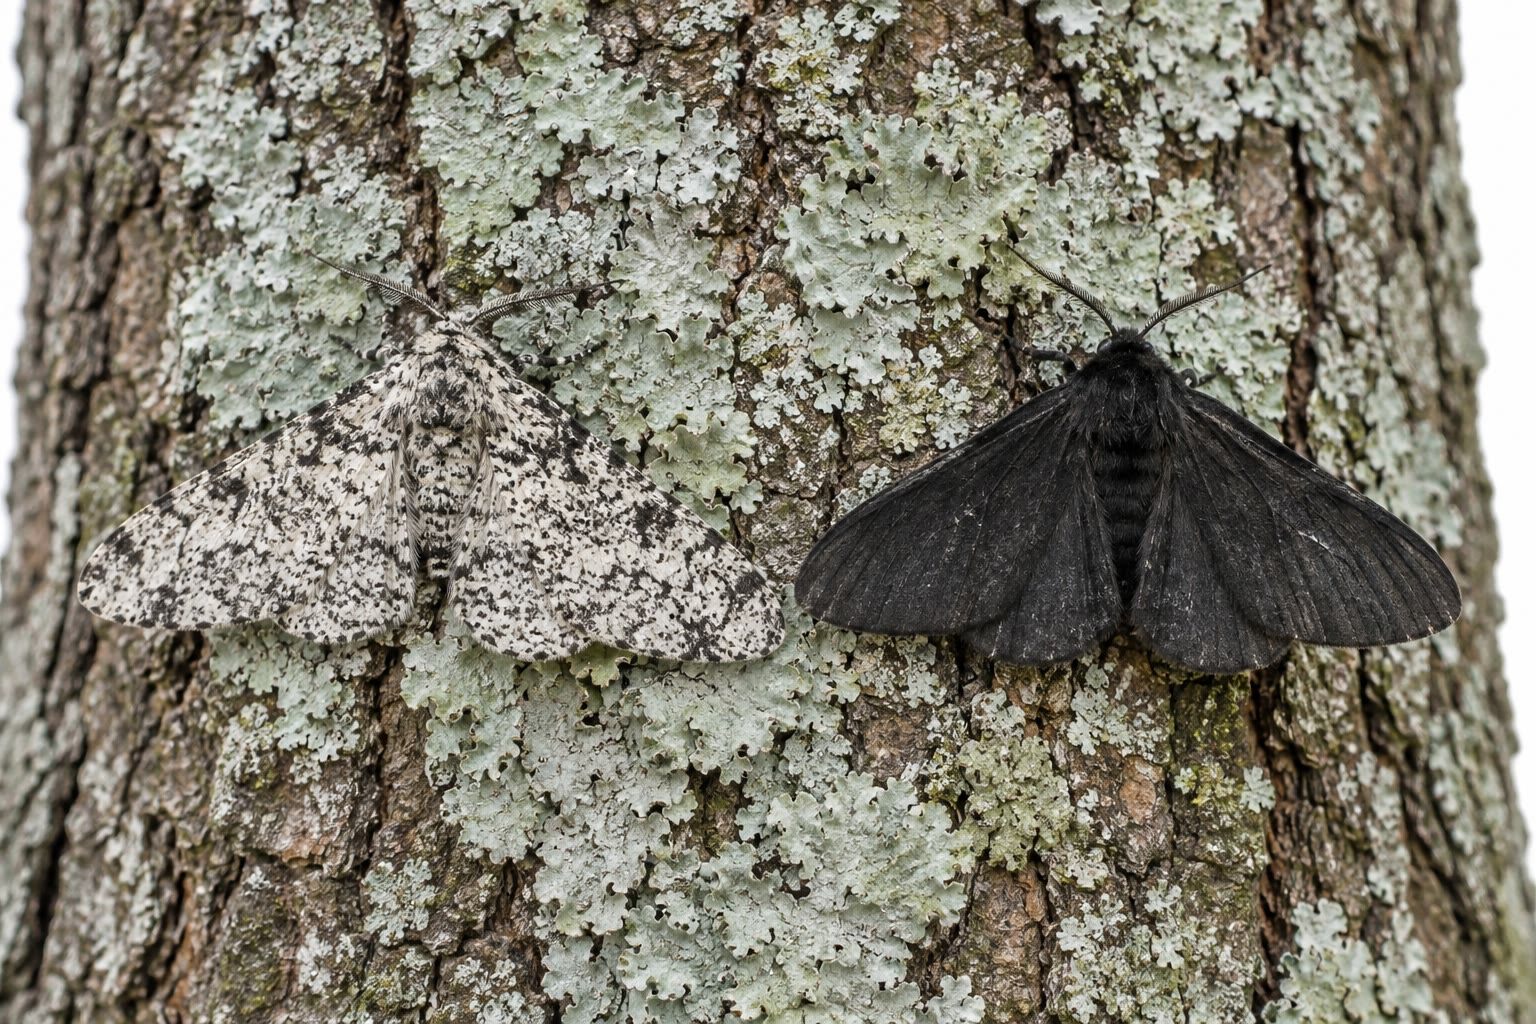
\includegraphics[width=0.46\linewidth]{images/book4/ai/b4-22-peppered-moths.jpg}\hspace{0.04\linewidth}
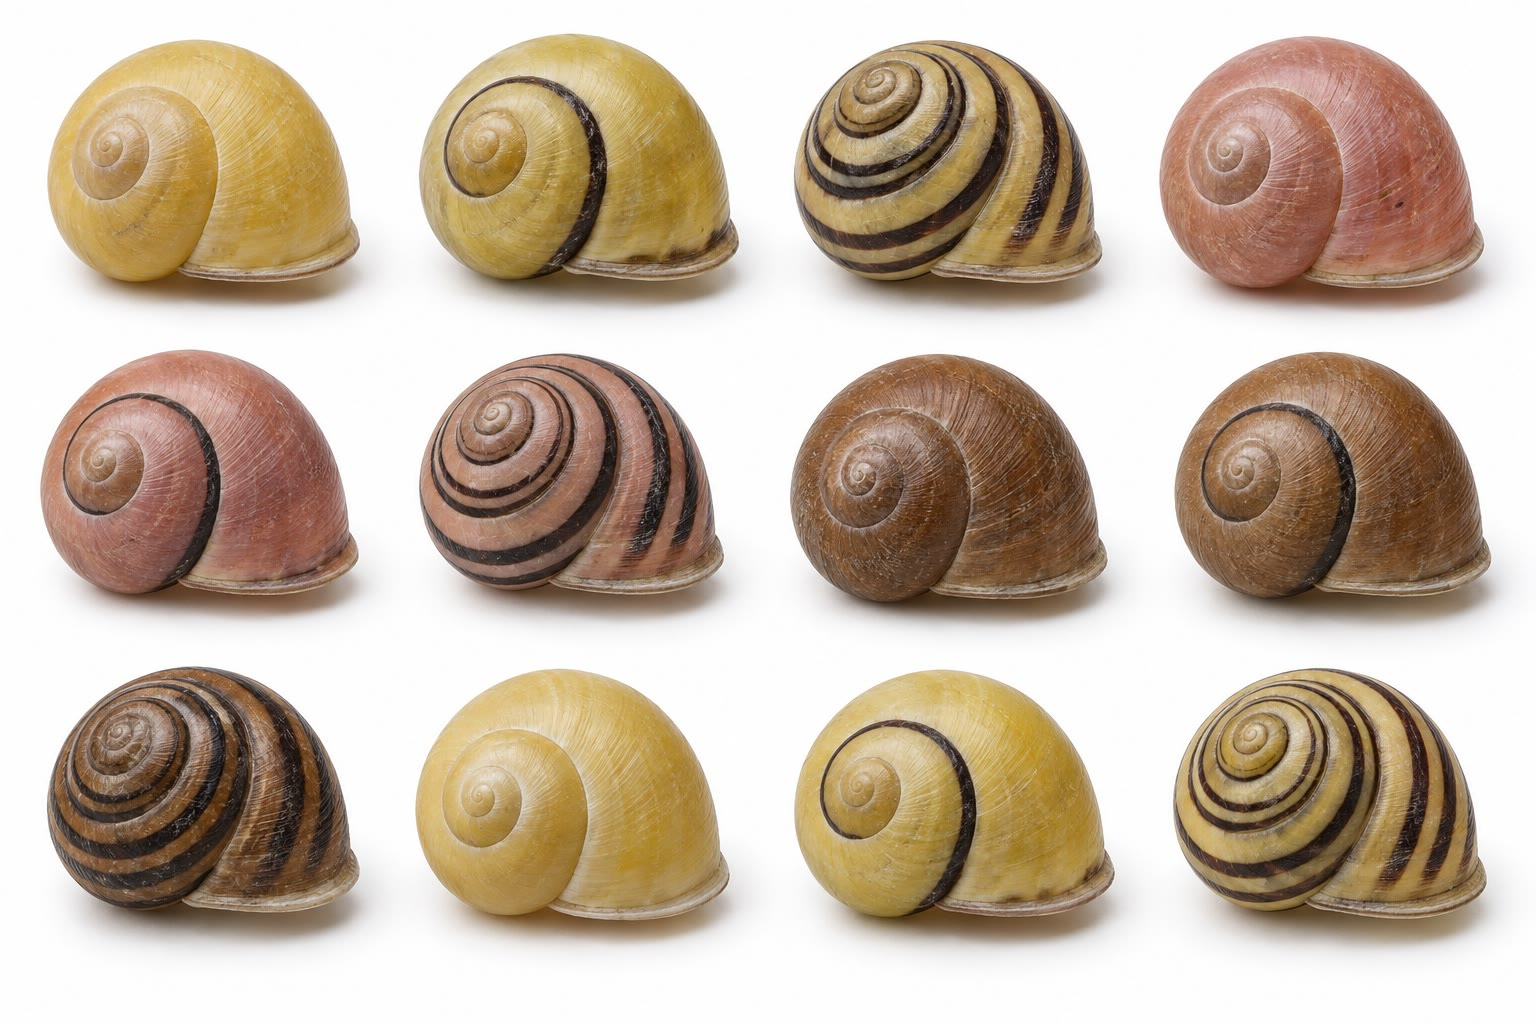
\includegraphics[width=0.46\linewidth]{images/book4/ai/b4-22-banded-snails.jpg}

{\small 左：停在地衣上的椒花蛾的两种型——
哪一种被鸟发现取决于\omterm{def:b2:plant-meristems:wood}{树皮}。右：林蜗牛壳的
多态现象，颜色和条纹在每个种群中得以保持，
依靠的是会学习识别常见型的捕食者。}
\end{omfigure}

\section{练习}

\begin{exercise}[$\star$]\label{exo:b2:population-genetics:1}
在 1000 人的样本中，640 人为 $MM$，320 人为 $MN$，40 人为 $NN$。
求\omterm{def:b2:population-genetics:frequencies}{等位基因频率}及哈代–温伯格期望。
该种群是否处于平衡状态？
\end{exercise}

\begin{exercise}[$\star$]\label{exo:b2:population-genetics:2}
白化病为\omterm{def:b2:meiosis-heredity:vocabulary}{隐性}遗传，每 \num{20000} 人中有一人患病。
求\omterm{def:b2:population-genetics:frequencies}{等位基因频率}及携带者频率。
\end{exercise}

\begin{exercise}[$\star$]\label{exo:b2:population-genetics:3}
定义\omterm{def:b2:population-genetics:fitness}{适合度}、\omterm{def:b2:population-genetics:fitness}{选择系数}和\omterm{thm:b2:population-genetics:heritability}{遗传力}，并列出
改变\omterm{def:b2:population-genetics:frequencies}{等位基因频率}的五种力。
\end{exercise}

\begin{exercise}[$\star$]\label{exo:b2:population-genetics:4}
各举一例说明\omterm{prop:b2:population-genetics:kinds}{定向选择}、\omterm{prop:b2:population-genetics:kinds}{稳定选择}和\omterm{prop:b2:population-genetics:kinds}{平衡选择}，
并指出每例的选择因子。
\end{exercise}

\begin{exercise}[$\star\star$]\label{exo:b2:population-genetics:5}
一个致死\omterm{def:b2:meiosis-heredity:vocabulary}{隐性}\omterm{def:b2:meiosis-heredity:vocabulary}{等位基因}的频率为 $0.02$。
使其减半需经过多少代？降至 $0.001$ 又需多少代？这说明
阻止患病个体繁殖有何作用？
\end{exercise}

\begin{exercise}[$\star\star$]\label{exo:b2:population-genetics:6}
已知 $w_{AA} = 1$，$w_{Aa} = 1$，$w_{aa} = 0.8$ 且 $p = 0.3$，求
$\bar w$、$p'$ 与 $\Delta p$。对 $p = 0.9$ 重复计算，
为何第二次的变化要小得多？
\end{exercise}

\begin{exercise}[$\star\star$]\label{exo:b2:population-genetics:7}
镰状细胞\omterm{def:b2:meiosis-heredity:vocabulary}{纯合}子的 $w = 0.2$，正常\omterm{def:b2:meiosis-heredity:vocabulary}{纯合}子的
$w = 0.88$，在疟疾流行区，\omterm{def:b2:meiosis-heredity:vocabulary}{杂合}子 $w = 1$。求
镰状\omterm{def:b2:meiosis-heredity:vocabulary}{等位基因}的平衡频率，以及
平衡时出生患该病的儿童所占比例。
\end{exercise}

\begin{exercise}[$\star\star$]\label{exo:b2:population-genetics:8}
一个\omterm{def:b2:meiosis-heredity:vocabulary}{隐性}致死基因由\omterm{def:b2:genome-diversification:mutation}{突变}产生，\omterm{def:b2:genome-diversification:mutation}{突变}率为 $\mu = \qty{2e-5}{}$
每个配子。求其平衡频率及
患病出生的比例。若\omterm{def:b2:meiosis-heredity:vocabulary}{显性}致死基因（生殖前致死）以相同\omterm{def:b2:genome-diversification:mutation}{突变}率产生，
则其出生比例为多少？
\end{exercise}

\begin{exercise}[$\star\star$]\label{exo:b2:population-genetics:9}
一个由 50 个繁殖个体组成的种群，初始 $H = 0.5$。
求其在 10、50 和 200 代后的\omterm{def:b2:meiosis-heredity:vocabulary}{杂合}度。要使种群
在 100 代内保留其\omterm{def:b2:meiosis-heredity:vocabulary}{杂合}度的 \qty{90}{\%}，
至少须多大？
\end{exercise}

\begin{exercise}[$\star\star\star$]\label{exo:b2:population-genetics:10}
一个岛屿被来自大陆种群的 10 只鸟定居，
该种群中某\omterm{def:b2:population-genetics:frequencies}{等位基因频率}为 $0.1$。求该\omterm{def:b2:meiosis-heredity:vocabulary}{等位基因}在奠基者中
缺失的概率，以及若其仅以一个拷贝存在于岛上，
则其最终在岛上被固定的概率。
并与大陆种群进行比较。
\end{exercise}

\begin{exercise}[$\star\star\star$]\label{exo:b2:population-genetics:11}
乳产量的 $h^{2} = 0.3$，标准差为
\qty{1000}{L}。育种者选留前 \qty{20}{\%} 的奶牛作为母本
（其平均值高于牛群均值 $1.4$ 个标准差）。
求每代的响应。若从前 
\qty{1}{\%} 中选取公牛（平均值高于牛群均值 $2.7$ 个标准差），响应为多少？
为何经过多代后响应会减缓？
\end{exercise}

\begin{exercise}[$\star\star\star$]\label{exo:b2:population-genetics:12}
“选择对其看不见的东西是盲目的。”试结合\omterm{def:b2:meiosis-heredity:vocabulary}{杂合}子中的\omterm{def:b2:meiosis-heredity:vocabulary}{隐性}\omterm{def:b2:meiosis-heredity:vocabulary}{等位基因}、
中性\omterm{def:b2:genome-diversification:mutation}{突变}，以及\omterm{thm:b2:population-genetics:heritability}{遗传力}为零的性状，
讨论选择能够作用于什么，
以及不能作用于什么。
\end{exercise}

\section{问题：飞蛾、岛屿与牛群}

\begin{problem}[{周末问题——由选择方程算得的椒花蛾兴起，
追踪奠基者种群的漂变与近交，
建立突变–选择平衡，
并预测育种计划，结尾落在
飞蛾的选择系数、岛屿的杂合度与牛群的增益}]
\label{pb:b2:population-genetics:1}
椒花蛾：黑化\omterm{def:b2:meiosis-heredity:vocabulary}{等位基因} $M$ 为\omterm{def:b2:meiosis-heredity:vocabulary}{显性}，频率 $p_0 = 0.001$
于 1848 年；50 代之后 \qty{90}{\%} 的飞蛾为黑化型；假设
$w_{MM} = w_{Mm} = 1$，$w_{mm} = 1 - s$。岛屿由 12 只鸟奠基，
其来源为 $H = 0.4$ 的大陆种群，一个\omterm{def:b2:meiosis-heredity:vocabulary}{隐性}有害
\omterm{def:b2:meiosis-heredity:vocabulary}{等位基因}的 $q = 0.05$；岛上此后保有
40 只繁殖个体。\omterm{def:b2:genome-diversification:mutation}{突变}率 $\mu = \qty{1e-5}{}$。牛群：$h^{2} = 0.4$，
标准差为 \qty{800}{L}。

\medskip
\noindent\textbf{第一部分——飞蛾。}
\begin{enumerate}
  \item 1848 年，黑化型飞蛾占多大比例，而
        $M$ \omterm{def:b2:meiosis-heredity:vocabulary}{等位基因}中有多大比例位于\omterm{def:b2:meiosis-heredity:vocabulary}{杂合}子中？
  \item 证明：当 $M$ 为\omterm{def:b2:meiosis-heredity:vocabulary}{显性}时，浅色\omterm{def:b2:meiosis-heredity:vocabulary}{等位基因}的频率
        服从 $q' = q(1 - sq)/(1 - sq^{2})$。
  \item 从 $q_0 = 0.999$ 出发，计算一代之后的 $q$，
        取 $s = 0.3$。
  \item \qty{90}{\%} 黑化意味着 $q^{2} = 0.1$，此时 $q$ 为多少？
  \item 用递推式逐步试算（或取近似式
        $\Delta q \approx -sq^{2}p$，并在 $q$ 接近 1 时使用），估计
        $s = 0.3$ 时使 $q$ 从 $0.999$
        降至 $0.32$ 所需的世代数，并与观察到的 50 代比较。
  \item 清洁空气法令实施后，浅色型获得优势，$s
        = 0.3$（相对于 $mm$），变为 $s = 0.3$（相对于 $M\_$）。证明
        $\Delta p = -spq^{2}/\bar w$，并解释浅色型的回归为何起初缓慢，
        而最终以 $M$ 的指数式衰减结束，
        而其兴起则起初呈指数式，
        其后却缓慢爬升。
\end{enumerate}

\medskip
\noindent\textbf{第二部分——岛屿。}
\begin{enumerate}[resume]
  \item 计算 12 只奠基者中没有一只携带
        有害\omterm{def:b2:meiosis-heredity:vocabulary}{等位基因}的概率。
  \item 计算奠基世代之后的期望\omterm{def:b2:meiosis-heredity:vocabulary}{杂合}度
        （由取自 $H = 0.4$ 的 12 个个体抽样而来，即 24 个
        基因拷贝）。
  \item 计算在 $N =
        40$ 时 100 代后的\omterm{def:b2:meiosis-heredity:vocabulary}{杂合}度，并以占大陆种群的比例表示。
  \item 一只鸟中出现一个中性\omterm{def:b2:genome-diversification:mutation}{突变}。计算其
        固定概率，以及若其会被固定时的
        期望固定时间。
  \item 岛上的鸟随机交配，但彼此皆有亲缘关系。若
        $F = 1/(2N)$ 每代累积，30 代后达到约 $0.3$，
        求患病\omterm{def:b2:meiosis-heredity:vocabulary}{纯合}子的频率，
        对 $q = 0.05$ 的\omterm{def:b2:meiosis-heredity:vocabulary}{等位基因}，分别计算有\omterm{prop:b2:population-genetics:inbreeding}{近交}与无\omterm{prop:b2:population-genetics:inbreeding}{近交}两种情形。
  \item 每一代都有一只来自大陆的鸟迁入。说明这对岛屿的
        \omterm{def:b2:cell-differentiation:differentiation}{分化}与其\omterm{thm:b2:population-genetics:balance}{遗传负荷}有何影响。
\end{enumerate}

\medskip
\noindent\textbf{第三部分——平衡。}
\begin{enumerate}[resume]
  \item 计算由\omterm{def:b2:genome-diversification:mutation}{突变}维持的\omterm{def:b2:meiosis-heredity:vocabulary}{隐性}\omterm{prop:b2:meiosis-heredity:extensions}{致死等位基因}的平衡频率，
        \omterm{def:b2:genome-diversification:mutation}{突变}率为 $\mu = 10^{-5}$，并求患病出生的比例。
  \item 对 $s = 0.1$ 的情形（一个轻度有害的
        \omterm{def:b2:meiosis-heredity:vocabulary}{隐性}\omterm{def:b2:meiosis-heredity:vocabulary}{等位基因}）计算同样的量。
  \item 计算\omterm{def:b2:meiosis-heredity:vocabulary}{显性}\omterm{def:b2:meiosis-heredity:vocabulary}{等位基因}的平衡，其\omterm{def:b2:meiosis-heredity:vocabulary}{杂合}子劣势为
        $hs = 0.05$。
  \item 医学治愈该致死病，使 $s$ 降至 $0.1$。平衡
        将如何变化，种群到达新平衡需要多长时间
        （数量级）？
  \item 基因组中有 \num{20000} 个基因，每个基因都会\omterm{def:b2:genome-diversification:mutation}{突变}为
        \omterm{def:b2:meiosis-heredity:vocabulary}{隐性}\omterm{prop:b2:meiosis-heredity:extensions}{致死等位基因}，\omterm{def:b2:genome-diversification:mutation}{突变}率为 $10^{-5}$。一个普通人平均携带多少个
        \omterm{prop:b2:meiosis-heredity:extensions}{致死等位基因}处于\omterm{def:b2:meiosis-heredity:vocabulary}{杂合}状态？（平衡时，每个基因座在每人
        体内有 $2\hat q$ 个拷贝。）
  \item 解释为何该数值与健康的种群相容，
        以及它为何使表亲通婚的代价高昂。
\end{enumerate}

\medskip
\noindent\textbf{第四部分——牛群。}
\begin{enumerate}[resume]
  \item 育种者选留前 \qty{30}{\%} 的奶牛（平均值
        比牛群高出 $1.16$ 个标准差）。计算以升为单位的选择差
        及其响应。
  \item 经过相同的选择五代之后，
        期望增益为多少，为何实际增益可能较小？
  \item 公牛提供一半的基因，并从前
        \qty{2}{\%}（$2.4$ 个标准差）中选出，计算
        奶牛与公牛按上述方式选择时的响应
        （取两种选择差的平均值）。
  \item 一个牛群中所有奶牛都是同一头动物的\omterm{def:b2:asexual-reproduction:clone}{克隆}，求
        $h^{2}$ 与响应各为多少？这说明了
        关于\omterm{thm:b2:population-genetics:heritability}{遗传力}的什么？
  \item 一个雀鸟种群的喙深具有 $h^{2} = 0.7$，干旱后幸存者
        的喙深高出 \qty{0.6}{mm}，预测
        下一代的情况。
  \item 育种者转而选择一个 $h^{2} = 0.1$ 的性状。需要多大的
        选择差（以标准差计）才能得到与
        第 19 题相同的响应？
  \item 给出结果：飞蛾的 $s$ 以及达到 \qty{90}{\%}
        黑化所需的时间，岛屿在 100 代后的\omterm{def:b2:meiosis-heredity:vocabulary}{杂合}度，
        以及牛群每代的响应。
\end{enumerate}
\end{problem}
